% sprint-review-wiring-tikz.tex
% Argument wiring diagram for sprint-review.tex.
% 28 nodes, 38 edges, following the AIF structure in sprint-review-wiring.json.
\begingroup
\footnotesize
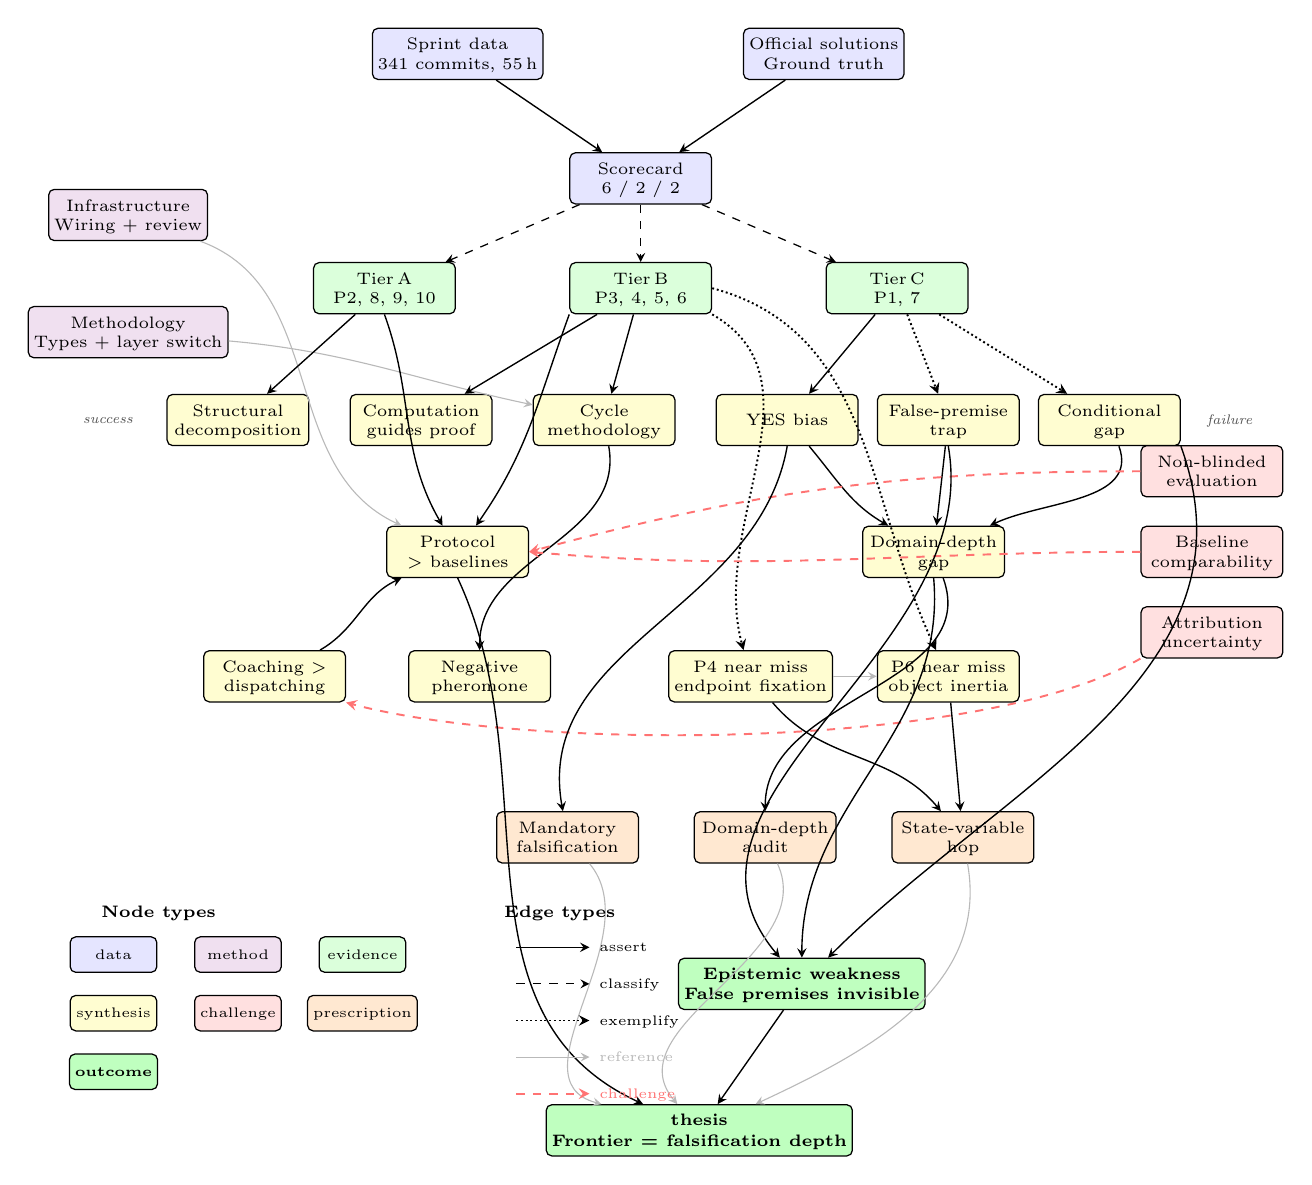
\begin{tikzpicture}[
  x=0.93cm,
  y=0.93cm,
  >=stealth,
  line width=0.45pt,
  text depth=0pt,
  box/.style={draw, rounded corners=2pt, align=center, inner sep=2pt,
              font=\fontsize{6}{7}\selectfont, minimum width=1.8cm,
              minimum height=0.65cm},
  data/.style={box, fill=blue!10},
  meth/.style={box, fill=violet!12},
  evid/.style={box, fill=green!14},
  synth/.style={box, fill=yellow!18},
  chall/.style={box, fill=red!12},
  presc/.style={box, fill=orange!18},
  outc/.style={box, fill=green!25,
               font=\fontsize{6.4}{7.4}\selectfont\bfseries},
  % Edge styles
  assert/.style={->, line width=0.5pt},
  classify/.style={->, dashed},
  exemp/.style={->, densely dotted, line width=0.7pt},
  refer/.style={->, gray!55, line width=0.4pt},
  challng/.style={->, red!55, dashed, line width=0.7pt},
  % Annotation
  annot/.style={font=\fontsize{5.5}{6.5}\selectfont\itshape,
                text=gray!65!black},
]

%% ═══════════════════════════════════════════════════════
%% LAYER 0 — Empirical base (y ≈ 16.5)
%% ═══════════════════════════════════════════════════════
\node[data] (D0) at (-2.5, 16.5) {Sprint data\\341 commits, 55\,h};
\node[data] (D1) at (2.5, 16.5) {Official solutions\\Ground truth};
\node[data] (D2) at (0, 14.8) {Scorecard\\6 / 2 / 2};

%% ═══════════════════════════════════════════════════════
%% METHODS (left margin)
%% ═══════════════════════════════════════════════════════
\node[meth] (M0) at (-7, 14.3) {Infrastructure\\Wiring + review};
\node[meth] (M1) at (-7, 12.7) {Methodology\\Types + layer switch};

%% ═══════════════════════════════════════════════════════
%% LAYER 2 — Tier decomposition (y ≈ 13.3)
%% ═══════════════════════════════════════════════════════
\node[evid] (TA) at (-3.5, 13.3) {Tier\,A\\P2, 8, 9, 10};
\node[evid] (TB) at (0, 13.3) {Tier\,B\\P3, 4, 5, 6};
\node[evid] (TC) at (3.5, 13.3) {Tier\,C\\P1, 7};

%% ═══════════════════════════════════════════════════════
%% LAYER 3 — Pattern identification (y ≈ 11.5)
%% ═══════════════════════════════════════════════════════
% Success (left)
\node[synth] (S1) at (-5.5, 11.5) {Structural\\decomposition};
\node[synth] (S2) at (-3, 11.5) {Computation\\guides proof};
\node[synth] (S3) at (-0.5, 11.5) {Cycle\\methodology};
% Failure (right)
\node[synth] (F1) at (2, 11.5) {YES bias};
\node[synth] (F2) at (4.2, 11.5) {False-premise\\trap};
\node[synth] (F3) at (6.4, 11.5) {Conditional\\gap};
% Side annotations
\node[annot, anchor=east] at (-6.8, 11.5) {success};
\node[annot, anchor=west] at (7.6, 11.5) {failure};

%% ═══════════════════════════════════════════════════════
%% LAYER 4 — Aggregated patterns (y ≈ 9.7)
%% ═══════════════════════════════════════════════════════
\node[synth] (S4) at (-2.5, 9.7) {Protocol\\$>$ baselines};
\node[synth] (F4) at (4, 9.7) {Domain-depth\\gap};

%% ═══════════════════════════════════════════════════════
%% LAYER 5 — Process + near misses (y ≈ 8.0)
%% ═══════════════════════════════════════════════════════
\node[synth] (P1) at (-5, 8.0) {Coaching $>$\\dispatching};
\node[synth] (P2) at (-2.2, 8.0) {Negative\\pheromone};
\node[synth] (N1) at (1.5, 8.0) {P4 near miss\\endpoint fixation};
\node[synth] (N2) at (4.2, 8.0) {P6 near miss\\object inertia};

%% ═══════════════════════════════════════════════════════
%% THREATS (right margin)
%% ═══════════════════════════════════════════════════════
\node[chall] (V1) at (7.8, 10.8) {Non-blinded\\evaluation};
\node[chall] (V2) at (7.8, 9.7) {Baseline\\comparability};
\node[chall] (V3) at (7.8, 8.6) {Attribution\\uncertainty};

%% ═══════════════════════════════════════════════════════
%% LAYER 6 — Prescriptions (y ≈ 5.8)
%% ═══════════════════════════════════════════════════════
\node[presc] (R1) at (-1, 5.8) {Mandatory\\falsification};
\node[presc] (R2) at (1.7, 5.8) {Domain-depth\\audit};
\node[presc] (R3) at (4.4, 5.8) {State-variable\\hop};

%% ═══════════════════════════════════════════════════════
%% LAYER 7 — Convergence (y ≈ 3.5–1.5)
%% ═══════════════════════════════════════════════════════
\node[outc] (C0) at (2.2, 3.8) {Epistemic weakness\\False premises invisible};
\node[outc] (C1) at (0.8, 1.8) {\textsc{thesis}\\Frontier = falsification depth};


%% ═══════════════════════════════════════════════════════
%% EDGES
%% ═══════════════════════════════════════════════════════

% --- Empirical base → scorecard ---
\draw[assert] (D0) -- (D2);
\draw[assert] (D1) -- (D2);

% --- Scorecard → tiers (classify) ---
\draw[classify] (D2) -- (TA);
\draw[classify] (D2) -- (TB);
\draw[classify] (D2) -- (TC);

% --- Methods → patterns (reference) ---
\draw[refer] (M0) to[out=-20, in=155] (S4);
\draw[refer] (M1) to[out=-5, in=168] (S3);

% --- Tier A → success ---
\draw[assert] (TA) -- (S1);
\draw[assert] (TA.south) to[out=-70, in=120] (S4);

% --- Tier B → success + near misses ---
\draw[assert] (TB) -- (S2);
\draw[assert] (TB) -- (S3);
\draw[assert] (TB.south west) to[out=-110, in=55] (S4);
\draw[exemp] (TB.south east) to[out=-30, in=105] (N1);
\draw[exemp] (TB.east) to[out=-15, in=115] (N2);

% --- Tier C → failure ---
\draw[assert] (TC) -- (F1);
\draw[exemp] (TC) -- (F2);
\draw[exemp] (TC) -- (F3);

% --- Failure → domain-depth gap ---
\draw[assert] (F1) to[out=-50, in=150] (F4);
\draw[assert] (F2) -- (F4);
\draw[assert] (F3) to[out=-70, in=25] (F4);

% --- Near misses ---
\draw[refer] (N1) -- (N2);
\draw[assert] (N1) to[out=-50, in=130] (R3);
\draw[assert] (N2) -- (R3);

% --- Process claims ---
\draw[assert] (P1) to[out=30, in=-155] (S4);
\draw[assert] (S3) to[out=-80, in=90] (P2);

% --- Threats challenge claims ---
\draw[challng] (V1.west) to[out=180, in=15] (S4.east);
\draw[challng] (V2.west) to[out=180, in=-5] (S4.east);
\draw[challng] (V3.south west) to[out=210, in=-15, looseness=0.6] (P1.south east);

% --- Failure → prescriptions ---
\draw[assert] (F1.south) to[out=-100, in=100] (R1);
\draw[assert] (F4) to[out=-70, in=90] (R2);

% --- Failure → epistemic weakness ---
\draw[assert] (F2.south) to[out=-80, in=130] (C0);
\draw[assert] (F3.south east) to[out=-70, in=45] (C0);
\draw[assert] (F4.south) to[out=-85, in=90] (C0);

% --- Convergence → thesis ---
\draw[assert] (S4.south) to[out=-65, in=155] (C1);
\draw[assert] (C0) -- (C1);
\draw[refer] (R1) to[out=-50, in=165] (C1);
\draw[refer] (R2) to[out=-65, in=130] (C1);
\draw[refer] (R3) to[out=-80, in=25] (C1);

%% ═══════════════════════════════════════════════════════
%% LEGEND
%% ═══════════════════════════════════════════════════════
\begin{scope}[shift={(-7.2, 1.0)}]
  \node[font=\fontsize{6.5}{7.5}\selectfont\bfseries,
        anchor=north west] at (-0.3, 4.0) {Node types};
  \node[data,  minimum width=1.1cm, minimum height=0.45cm]
       at (0, 3.2) {\fontsize{5.2}{6}\selectfont data};
  \node[meth,  minimum width=1.1cm, minimum height=0.45cm]
       at (1.7, 3.2) {\fontsize{5.2}{6}\selectfont method};
  \node[evid,  minimum width=1.1cm, minimum height=0.45cm]
       at (3.4, 3.2) {\fontsize{5.2}{6}\selectfont evidence};
  \node[synth, minimum width=1.1cm, minimum height=0.45cm]
       at (0, 2.4) {\fontsize{5.2}{6}\selectfont synthesis};
  \node[chall, minimum width=1.1cm, minimum height=0.45cm]
       at (1.7, 2.4) {\fontsize{5.2}{6}\selectfont challenge};
  \node[presc, minimum width=1.1cm, minimum height=0.45cm]
       at (3.4, 2.4) {\fontsize{5.2}{6}\selectfont prescription};
  \node[outc,  minimum width=1.1cm, minimum height=0.45cm]
       at (0, 1.6) {\fontsize{5.2}{6}\selectfont outcome};

  \node[font=\fontsize{6.5}{7.5}\selectfont\bfseries,
        anchor=north west] at (5.2, 4.0) {Edge types};
  \draw[assert]  (5.5, 3.3) -- (6.5, 3.3)
       node[right, font=\fontsize{5.2}{6}\selectfont] {assert};
  \draw[classify] (5.5, 2.8) -- (6.5, 2.8)
       node[right, font=\fontsize{5.2}{6}\selectfont] {classify};
  \draw[exemp]   (5.5, 2.3) -- (6.5, 2.3)
       node[right, font=\fontsize{5.2}{6}\selectfont] {exemplify};
  \draw[refer]   (5.5, 1.8) -- (6.5, 1.8)
       node[right, font=\fontsize{5.2}{6}\selectfont] {reference};
  \draw[challng] (5.5, 1.3) -- (6.5, 1.3)
       node[right, font=\fontsize{5.2}{6}\selectfont] {challenge};
\end{scope}

\end{tikzpicture}
\endgroup
